%%%%%%%%%%%%%%%%%%%%%%%%%%%%%%%%%%%%%%
% LaTeX poster template
% Created by Nathaniel Johnston
% August 2009
% http://www.nathanieljohnston.com/2009/08/latex-poster-template/
%%%%%%%%%%%%%%%%%%%%%%%%%%%%%%%%%%%%%%

\documentclass[final, table]{beamer}
%\usepackage[scale=1.24]{beamerposter}
\usepackage[size=a1,scale=1.1]{beamerposter}
\usepackage{graphicx}			% allows us to import images
\usepackage{subfigure}

%-----------------------------------------------------------
% Define the column width and poster size
% To set effective sepwid, onecolwid and twocolwid values, first choose how many columns you want and how much separation you want between columns
% The separation I chose is 0.024 and I want 4 columns
% Then set onecolwid to be (1-(4+1)*0.024)/4 = 0.22
% Set twocolwid to be 2*onecolwid + sepwid = 0.464
%-----------------------------------------------------------

\newlength{\sepwid}
\newlength{\onecolwid}
\newlength{\twocolwid}
\newlength{\threecolwid}
\setlength{\paperwidth}{48in}
\setlength{\paperheight}{42in}
%\setlength{\paperwidth}{42in}
%\setlength{\paperheight}{36in}
\setlength{\sepwid}{0.024\paperwidth}
\setlength{\onecolwid}{0.22\paperwidth}  % For 4 columns
%\setlength{\onecolwid}{0.30\paperwidth}   % 3 columns
\setlength{\twocolwid}{0.464\paperwidth}
\setlength{\threecolwid}{0.708\paperwidth}
\setlength{\topmargin}{-0.5in}
\usetheme{confposter}
\usepackage{exscale}
\usepackage[font=singlespacing]{caption}
\usepackage{multirow}

%-----------------------------------------------------------
% The next part fixes a problem with figure numbering. Thanks Nishan!
% When including a figure in your poster, be sure that the commands are typed in the following order:
% \begin{figure}
% \includegraphics[...]{...}
% \caption{...}
% \end{figure}
% That is, put the \caption after the \includegraphics
%-----------------------------------------------------------

%\usecaptiontemplate{
%\small
%\structure{\insertcaptionname~\insertcaptionnumber:}
%\insertcaption}
\setbeamertemplate{caption}[numbered]

%-----------------------------------------------------------
% Define colours (see beamerthemeconfposter.sty to change these colour definitions)
%-----------------------------------------------------------

\setbeamercolor{block title}{fg=dblue,bg=white}
\setbeamercolor{block body}{fg=black,bg=white}
\setbeamercolor{block alerted title}{fg=white,bg=dblue!70}
\setbeamercolor{block alerted body}{fg=black,bg=dblue!10}

%-----------------------------------------------------------
% Math commands
%-----------------------------------------------------------
\newcommand{\X}{\mathcal{X}}
\newcommand{\Y}{\mathcal{Y}}
\newcommand{\G}{\mathcal{G}}
\newcommand{\norm}[1]{\left | \left | #1 \right | \right |}
\newcommand{\reals}{\mathbb{R}}
\newcommand{\scrF}{\mathcal{F}}
\newcommand{\E}{\mathbb{E}}
\newcommand{\K}{\mathcal{K}}
\newcommand{\PP}{\mathbb{P}}
\newcommand{\N}{\mathbb{N}}
\newcommand{\Dir}{\text{Dir}}
\newcommand{\DP}{\text{DP}}
\newcommand{\Pois}{\text{Pois}}
\newcommand{\BP}{\text{BP}}
\newcommand{\BeP}{\text{BeP}}
\newcommand{\borel}{\mathcal{B}}
\newcommand{\Beta}{\text{Beta}}
\newcommand{\Discrete}{\text{Discrete}}
\newcommand{\Ber}{\text{Bernoulli}}
\newcommand{\CRP}{\text{CRP}}
\newcommand{\IBP}{\text{IBP}}
\newcommand{\Norm}{\text{N}}
\newcommand{\B}{\mathcal{B}}
\newcommand{\Corr}{\text{Corr}}
\newcommand{\Un}{\text{Un}}
\newcommand{\CRM}{\text{CRM}}
\newcommand{\NiG}{\text{NiG}}
\newcommand{\Cat}{\text{Cat}}
\newcommand{\T}{\mathcal{T}}
\newcommand{\Ga}{\text{Ga}}
\newcommand{\notrightarrow}{\centernot\rightarrow}
\newcommand{\gap}{\text{    }}



%-----------------------------------------------------------
% Name and authors of poster/paper/research
%-----------------------------------------------------------

\title{Automated Antibody Characterization for Array Tomography}
\author{
Anish K. Simhal		\textsuperscript{1*},
Belvin Gong			\textsuperscript{2},
James S. Trimmer		\textsuperscript{2},
Richard J. Weinberg		\textsuperscript{3},
Stephen J. Smith		\textsuperscript{4}, \\
Guillermo Sapiro		\textsuperscript{1, 5}, 
Kristina D. Micheva		\textsuperscript{6}}
\institute{\textsuperscript{1}Electrical and Computer Engineering, Duke University 
\textsuperscript{2} Dept. of Neurobiology, University of California, Davis \\
\textsuperscript{3} Dept. of Cell Biology and Physiology, University of North Carolina
\textsuperscript{4} Synapse Biology, Allen Institute for Brain Sciences \\
\textsuperscript{5} Dept. of Biomedical Engineering, Dept. of Computer Science, Dept. of Mathematics, Duke University \\
\textsuperscript{6} Molecular and Cellular Physiology, Stanford University School of Medicine}

%-----------------------------------------------------------
% Start the poster itself
%-----------------------------------------------------------
\begin{document} 
\addtobeamertemplate{headline}{} 
{\begin{tikzpicture}[remember picture, overlay]
\node [anchor=north west, inner sep=3cm]  at (current page.north west)
{
\includegraphics[scale=0.225]{figs/duke_univ_blue}};
\end{tikzpicture}
\vspace{6cm} %twiddle with this later...
\begin{tikzpicture}[remember picture, overlay]
\node [anchor=north east, inner sep=3cm]  at (current page.north east)
{
\includegraphics[scale=0.55]{figs/IID_logo}};
\end{tikzpicture}
}
\begin{frame}[t]  
\begin{columns}[t]  % align column content at top

% First column
\begin{column}{\sepwid}\end{column}  % spacer column
\begin{column}{\onecolwid} 

\begin{block}{Challenge} 

\begin{itemize} 
\item \textbf{How to quantify antibody performance for array tomography? }
\end{itemize} 


\begin{figure}
\centering
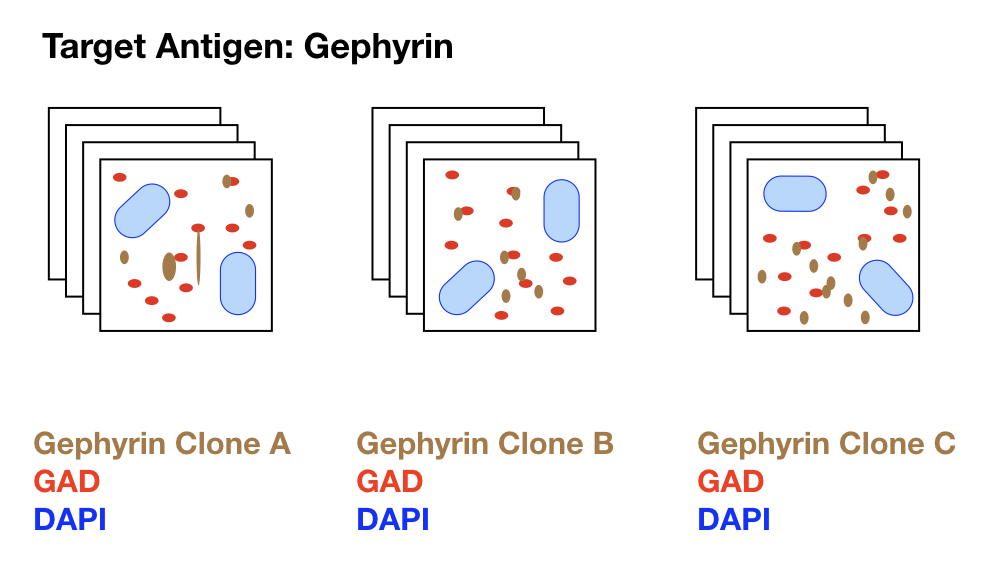
\includegraphics[width=0.9\textwidth]{figs/issuesWithAntibodies}
\caption{Each set of squares represents a 3D tomographic array of images from mouse cortex. The large blue blobs represent DAPI.  The red dots represent GAD immunostaining, using a previously validated antibody. The brown dots represent the gephyrin antibody clone of interest. }
\label{fig:issueswithantibodies}
\end{figure}


\begin{figure}
\centering
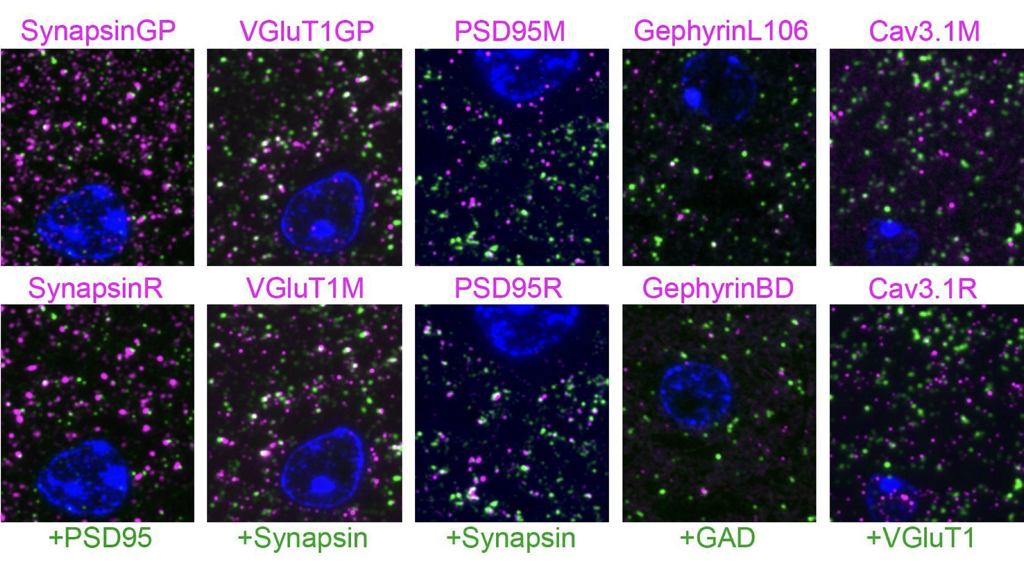
\includegraphics[width=0.9\textwidth]{figs/pairwise}
\caption{Pairwise comparison of immunofluorescence signals on single sections from mouse brain. Each column represents an experiment where two antibodies against the same antigen (magenta) are evaluated by co-labeling with a control antibody (green). The sections are also labeled with the nuclear stain DAPI (blue).}
\label{fig:pariwise}
\end{figure}

\end{block}

\begin{block}{Background} 

\begin{itemize} 
\item \textbf{Array Tomography Pipeline}
\end{itemize} 

\begin{figure}
\centering
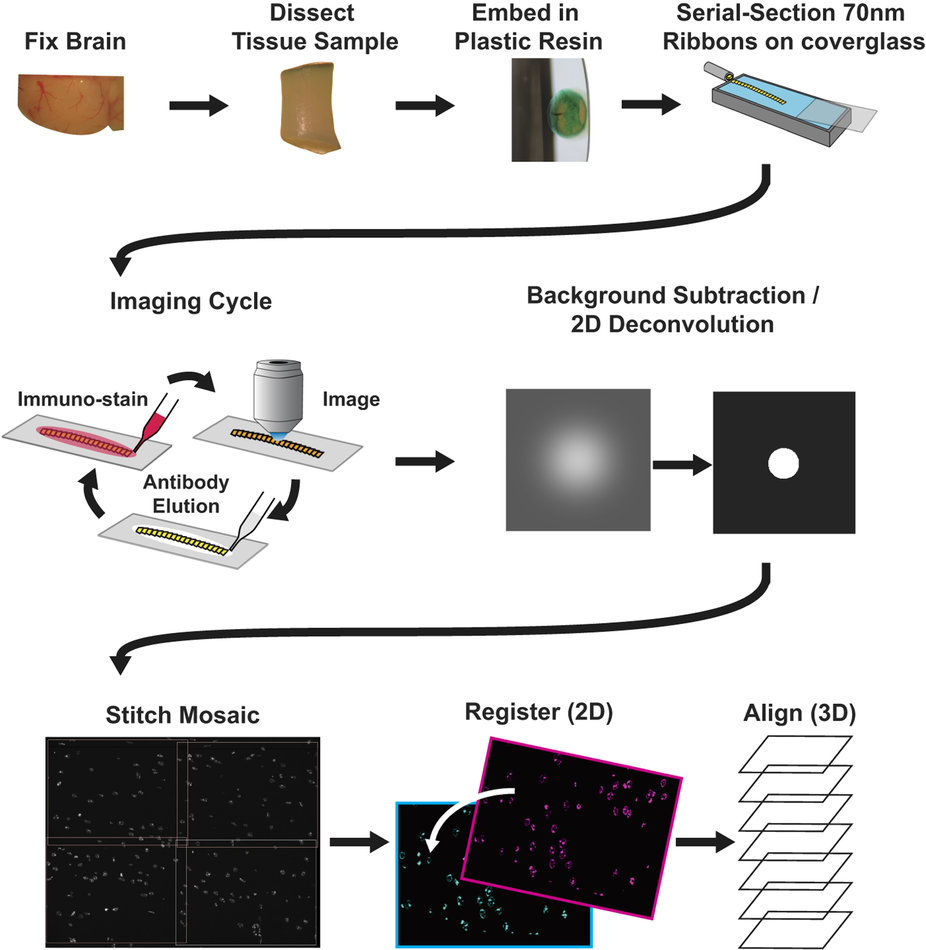
\includegraphics[width=0.8\textwidth]{figs/at_diagram3}
\caption{Array Tomography (AT) methodology used for creating the data \cite{Weiler}}
\end{figure}




\end{block} 


\end{column}

% Second column
\begin{column}{\sepwid}\end{column}  % spacer column
\begin{column}{\twocolwid}




\begin{block}{Action}

\textbf{Method Overview}

\begin{itemize} 
\item Compute a series of quantitative measurements using a probabilistic query-based synapse detector to evaluate and compare different antibodies and antibody dilutions.  
%
%The measurements are selected to provide unbiased quantitative information to help evaluate the specificity and sensitivity of antibodies. By comparing the performance of different antibodies against a single antigen, we use the approach to identify antibodies well-suited for array tomography on brain sections
\end{itemize} 

\begin{figure}
\centering

\includegraphics[width=0.9\textwidth]{figs/ABWorkflow}
\caption{Pipeline of the proposed automatic antibody characterization and screening method}
\label{fig:pipeline}
\end{figure}


\begin{columns}[t]  % align column content at top

\begin{column}{\onecolwid}


\textbf{Measure 1: Detected Density of Puncta} 

\begin{itemize} 
\item Reflects the sensitivity and selectivity of the antibody at the concentration used
\end{itemize} 

\begin{figure}
\centering
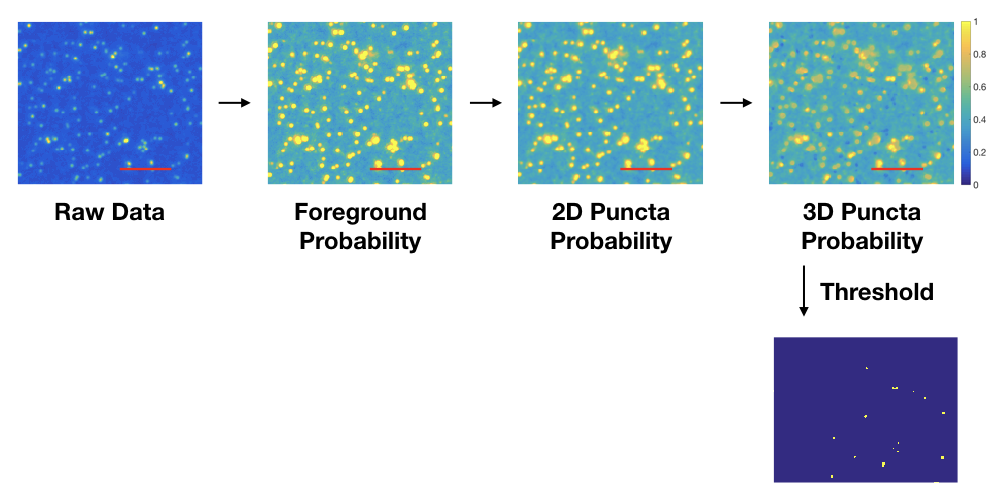
\includegraphics[width=1\textwidth]{figs/3dpuncta_pipeline}
\caption{The first box shows the raw image data. The second box is the output of a 'foreground probability' step; the intensity value of each pixel codes the probability it belongs to the foreground.  The third box is the output of a '2D Puncta Probability' step; each pixel codes the probability that it belongs to a 2D blob; the thresholded result is shown below.  The '3D puncta probability' image's intensity values are the probability that a voxel belongs to a blob which spans the minimum number of slices.  Second Row: the thresholded output of the 3D probability map.} 
\end{figure}

\textbf{Measure 2: Puncta Volume Size \& Standard Deviations} 

\begin{itemize} 
\item Reflects the quality and consistency of the antibody staining
\end{itemize} 


\begin{figure}
\centering
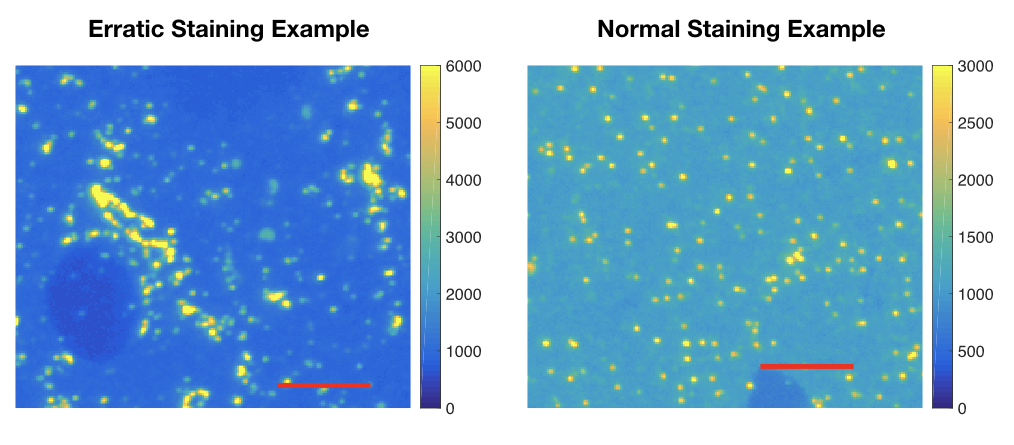
\includegraphics[width=1\textwidth]{figs/ab_sizevariance}
\caption{Left) Staining for collybistin on a raw IF slice; note the very broad distribution of sizes for puncta. (Right) Relatively 'normal' pattern of staining on a raw IF slice, using a different anti-collybistin clone.  This difference is automatically quantified by the proposed framework. Each red scale bar is 5$\mu m$.} 

\end{figure}




\end{column}

% Third column

\begin{column}{\sepwid}\end{column}  % spacer column
\begin{column}{\onecolwid}

\textbf{Measure 3: Synapse Density} 
\begin{itemize} 
\item Useful for evaluating antibodies against targets with a known distribution at synapses, where the density of synapses containing the target protein can be estimated.
\end{itemize} 


\begin{figure}
\centering
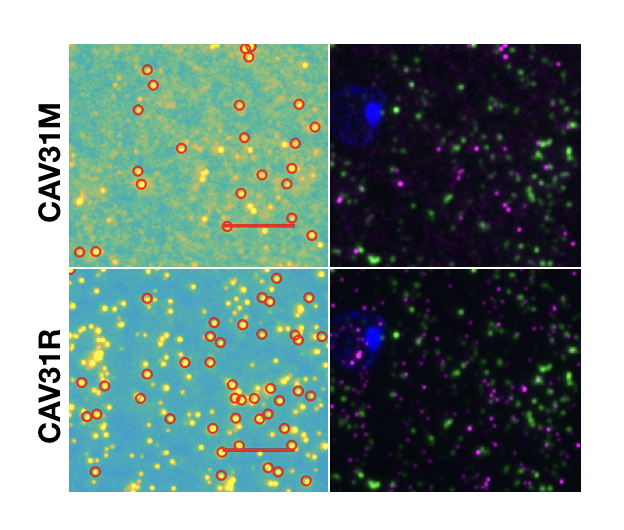
\includegraphics[width=0.8\textwidth]{figs/synapsedetection}
\caption{Pairwise comparison of CAV31 IF signals on single sections from mouse brain.  The images in the left column show color scaled IF images with synapse detections overlaid in red.  The right column shows the 3 IF channels collated - CAV31 (purple), VGluT1 (green), \& DAPI (blue)} 
\end{figure}


\textbf{Measure 4: Antibody Staining Precision} 

\begin{itemize} 
\item Estimates the magnitude of 'extra' (nonsynaptic) staining. When comparing two antibodies against the same target, differences in precision are likely to reflect differences in their specificity.  \end{itemize} 


\begin{figure}
\centering
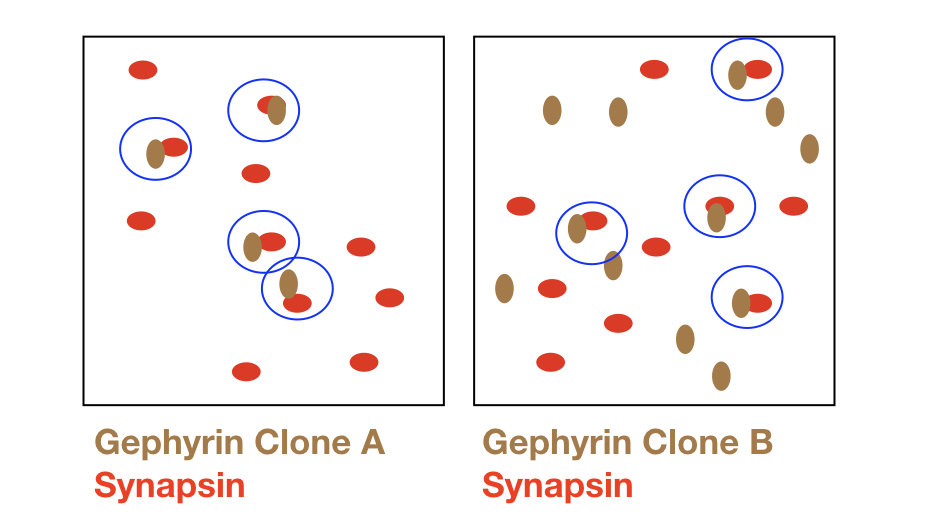
\includegraphics[width=1\textwidth]{figs/ab_precision_cartoon}
\caption{In the left panel, each gephyrin punctum lies adjacent to a synapsin puncta, indicating a synapse.  The right panel shows multiple gephyrin punctum unassociated with synapsin puncta, indicating possible poor specificity. } 
\end{figure}


\end{column}
\end{columns} 
\end{block}
\end{column} 

% Fourth column
\begin{column}{\sepwid}\end{column}  % spacer column
\begin{column}{\onecolwid}

\begin{block}{Resolution} 

\textbf{Pairwise Antibody Comparisons} 


\begin{figure}
\centering
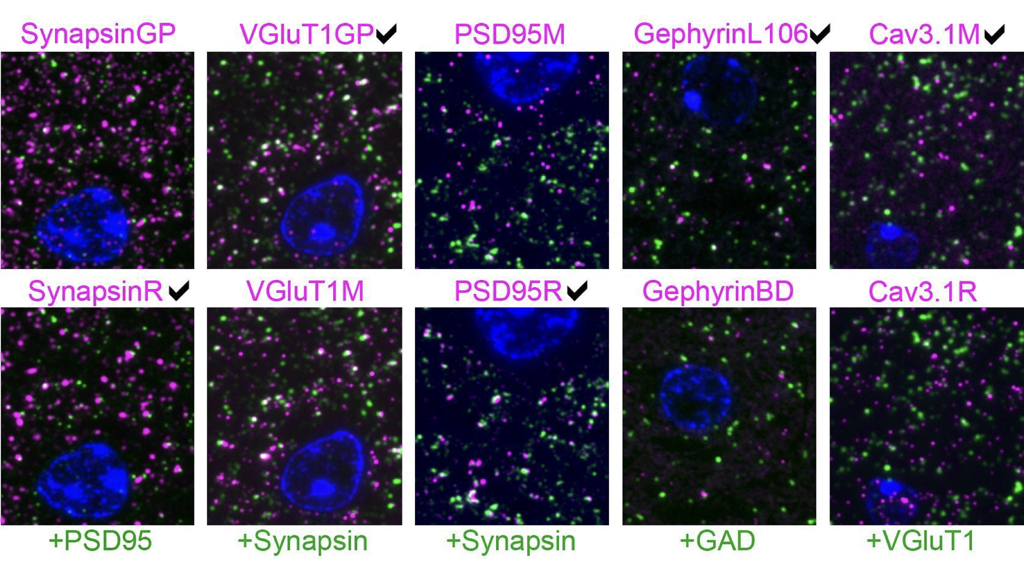
\includegraphics[width=0.8\textwidth]{figs/pairwise_check}
\caption{Image from Figure \ref{fig:pairwise_check} with checkmarks indicating the superior antibody. The better antibody is judged to be the one that has more puncta associated with the control antibody and fewer puncta not associated with the control antibody. Each image is 16$x$18$\mu m$. }
\label{fig:pairwise_check}
\end{figure}


\begin{figure}
\centering
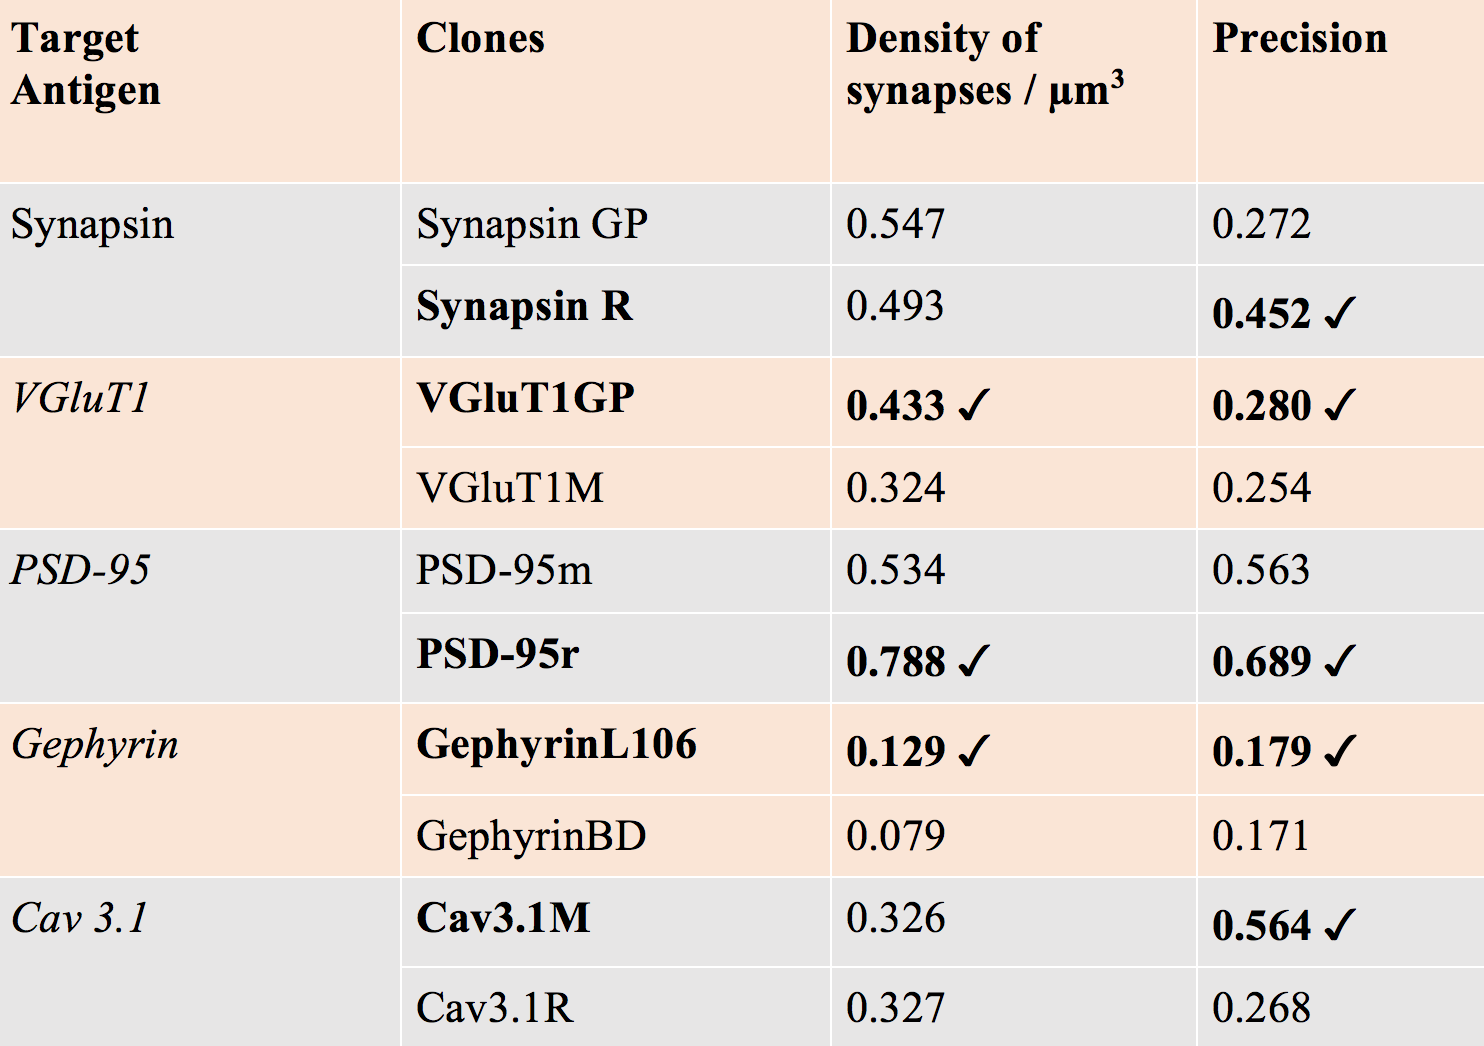
\includegraphics[width=0.9\textwidth]{figs/pairwise_table}
\caption{Results from pairwise antibody comparisons, as shown in Figure \ref{fig:pairwise_check}.  The name in bold represents the antibody preferred by an expert based on visual examination.  Check marks are placed next to the measurements used to determine the optimal antibody.}
\label{fig:pairwise_table}
\end{figure}

\textbf{Comparing Multiple Antibody Clones} 


\begin{figure}
\centering
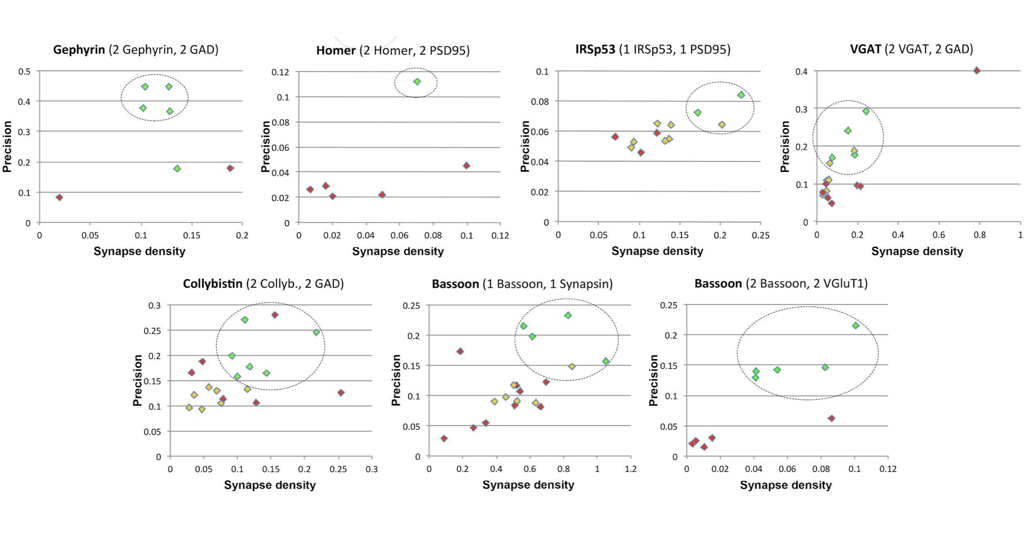
\includegraphics[width=1\textwidth]{figs/multiple_clones_graphs}
\caption{Each scatter plot shows the synapse density and precision scores of multiple clones of the same antibody, with the best ranking clones circled. Expert ranking is color coded: green - best, orange - unclear, red - fail. The specific query in each case is indicated in the plot title, where the number indicates the minimum punctum size for each label.  }
\label{fig:multiple_clones_graphs}
\end{figure}
% For example, '2 Gephyrin, 2 GAD' means that a synapse in this case is defined as a gephyrin punctum that spans at least 2 slices adjacent to a GAD punctum that also spans at least 2 slices.
\end{block} 

\begin{block}{Acknowledgments} 

\tiny{This work was supported by the National Institutes of Health (NIH-TRA 1R01NS092474), the Allen Institute for Brain Sciences (AIBS), and the Information Initiative at Duke University}
\end{block} 


\vspace{-0.05in}
\begin{block}{References}
\tiny{
\begin{thebibliography}{99}


\bibitem{Micheva2} 
Micheva KD, Smith SJ. Array tomography: a new tool for imaging the molecular architecture and ultrastructure of neural circuits. Neuron. 2007 Jul 5;55(1):25-36.

\bibitem{Saber} Saper CB. A guide to the perplexed on the specificity of antibodies. Journal of Histochemistry \& Cytochemistry. 2009;57(1):1-5.

\bibitem{Simhal} 
Simhal, Anish K., et al. Probabilistic Fluorescence-Based Synapse Detection. PLoS Computational Biology, May 2017.

\bibitem{Weiler} 
Weiler NC, Collman F, Vogelstein JT, Burns R, Smith SJ. Synaptic molecular imaging in spared and deprived columns of mouse barrel cortex with array tomography. Scientific Data. 2014 Dec 23;1.

\end{thebibliography}}
\end{block}

\end{column}


\end{columns}
\end{frame}
\end{document}
